\chapter{KMeans, GMM, FCM compare figures}

\begin{figure}[h]
    \centering
    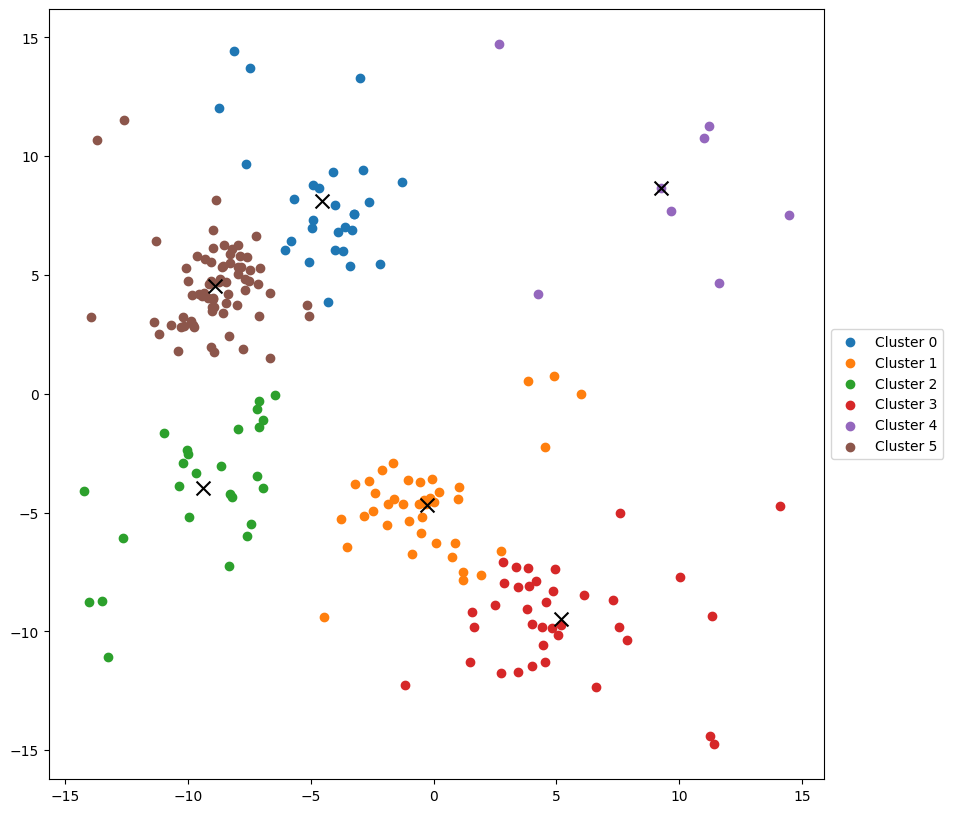
\includegraphics[width=0.9\linewidth]{Figures/dati_kmeans.png}
    \caption[example of \gls{kmeans} clustering]{The data points are coloured according to the calculated label and the estimated centroid is indicated with a \texttt{X}.}
    \label{fig:data_kmeans}
\end{figure}
\begin{figure}[h]
    \centering
    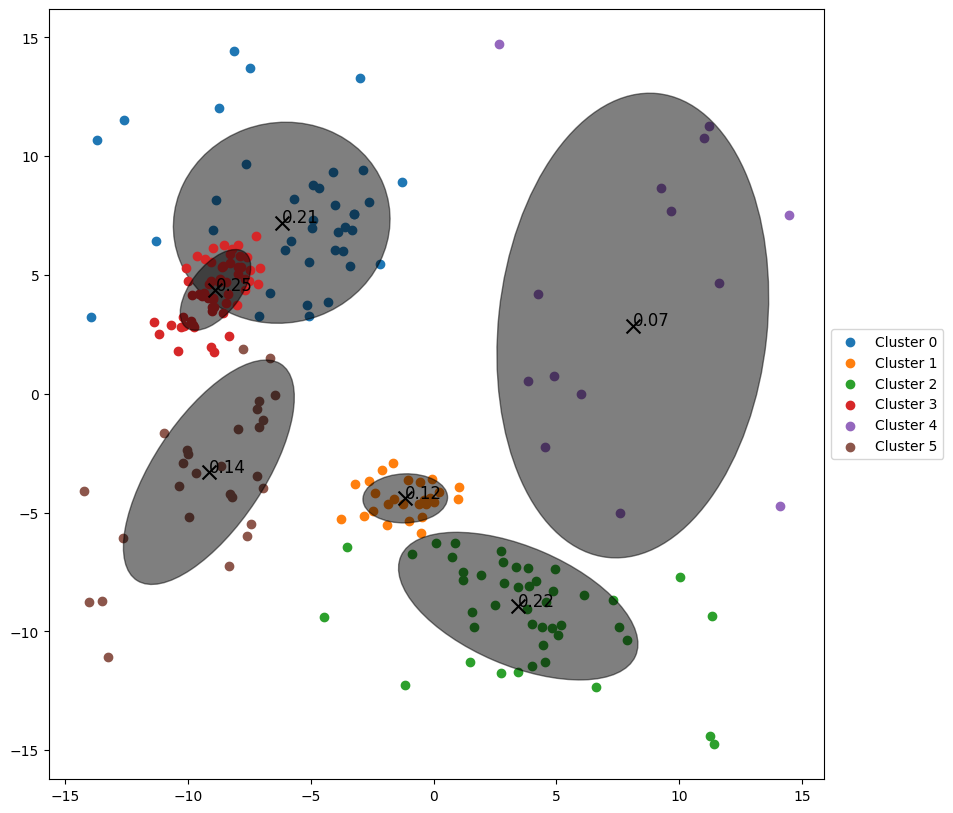
\includegraphics[width=0.9\linewidth]{Figures/dati_gmm.png}
    \caption[example of \gls{gmm} clustering]{The data points are coloured according to the Mahalanobis distance and the estimated centroid is indicated with a \texttt{X}. The ellipse of the normal distribution represents the covariance and is a confidence region of $95\%$.}
    \label{fig:data_gmm}
\end{figure}
\begin{figure}[h]
    \centering
    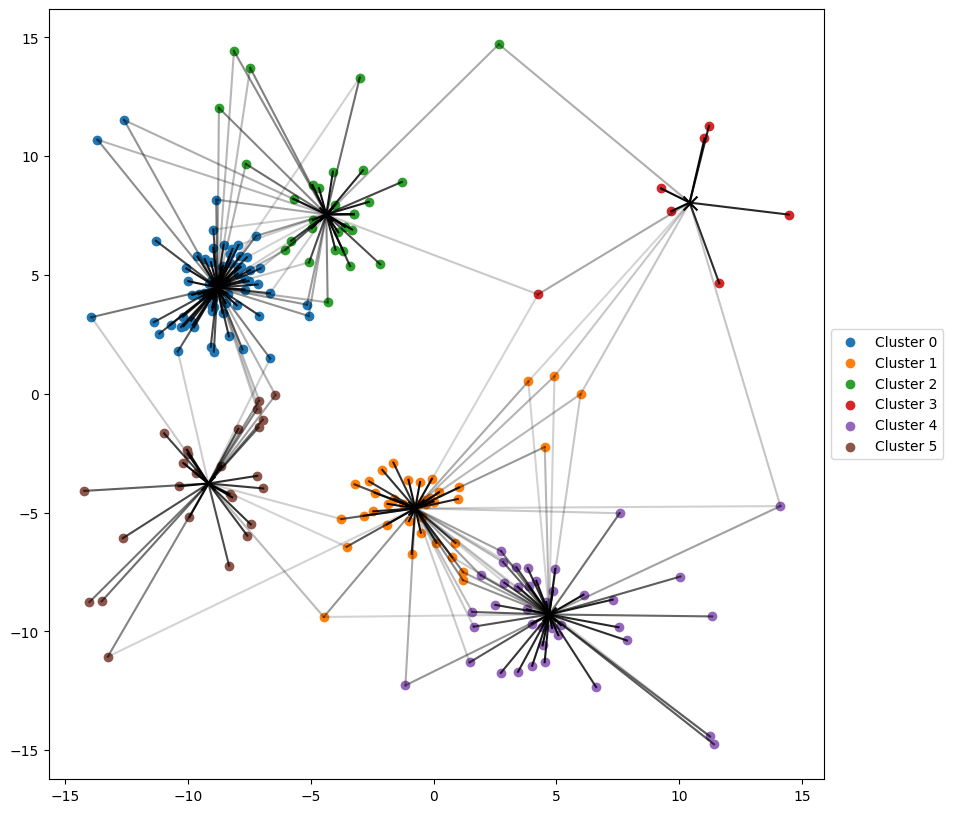
\includegraphics[width=0.9\linewidth]{Figures/dati_fcm.png}
    \caption[example of \gls{fcm} clustering]{The data points are coloured according to the most probable label and the estimated centroid is indicated with a \texttt{X}. The lines indicate the assignments with the greatest degree of affiliation of each point to the clusters; the darker the lines, the stronger the assignment.}
    \label{fig:data_fcm}
\end{figure}

\chapter{FCM implementation with CUDA}
\gls{cuda} è un'architettura hardware supportata dai processori grafici di \emph{NVIDIA}, un'azienda statunitense. E' possibile realizzare il codice che definisce la comunicazione tra \gls{cpu} e \gls{gpu} in un dialetto del \gls{cxx}. Il codice che effettivamente esegue il processore grafico può essere già implementato con funzioni speciali delle librerie \gls{thrust} e \gls{cuBLAS} o realizzato personalmente attraverso dei kernel. In questa appendice si mostra il kernel usato per realizzare il calcolo della matrice $U^2$ in \gls{fcm}. In particolare l'algoritmo è ottimizzato per compiere il calcolo su al più MAX\_THREAD\_PER\_BLOCK centroidi, poiché nel medesimo

\begin{lstlisting}[style=code, language=C, rulecolor=\color{blue}]
/**
 * @brief This kernel computes the matrix U2 of membership between
 * data points and centroids
 *
 * @param[in] d_data : the i-th is d_data[i * n_dimensions + k]
 * for k = 0, ..., n_dimensions - 1
 * @param[in] d_weights : the weight of the i-th data point is
 * d_weights[i]
 * @param[in] d_centroids : the j-th is
 * d_centroids[j * n_dimensions + k] for k = 0, ..., n_dimensions - 1
 * @param[out] d_matrix : the weighted membership between the i-th data point
 * and the j-th centroid is stored in d_matrix[i * n_centroids + j]
 * @param n_data : number of data points
 * @param n_dimensions : dimensions of data points
 * @param n_centroids : number of centroids
 *
 * @details This kernel requires a grid of blocks with n_data blocks
 * and MAX_THREADS_PER_BLOCK threads for each block.
 *
 * @note This kernel synchronize threads at the end of the computation
 */
__global__ void
kernel_compute_U2 (const float *const d_data, const float *const d_weights,
const float *const d_centroids, float *const d_matrix,
size_t n_data, size_t n_dimensions, size_t n_centroids)
{
  __shared__ float sdata[MAX_THREADS_PER_BLOCK];
  size_t i = blockIdx.x;  // i-th data
  size_t j = threadIdx.x; // j-th centroid
  float value = 0;
  float min_value = 0;
  // compute the distance between the i-th data point and the j-th
  // centroid
  if (i < n_data && j < n_centroids)
    {
      for (size_t k = 0; k < n_dimensions; k++)
        {
          float diff = d_data[i * n_dimensions + k]
                     - d_centroids[j * n_dimensions + k];
          value += diff * diff;
        }
    }
  // syncronyze threads of this block
  __syncthreads ();
  // compute the min value of the block
  if (j < n_centroids)
  sdata[j] = value;
  else
  sdata[j] = FLT_MAX;
  __syncthreads ();
  for (size_t s = MAX_THREADS_PER_BLOCK / 2; s > 0; s >>= 1)
    {
      if (j < s && sdata[j] > sdata[j + s])
      sdata[j] = sdata[j + s];
      __syncthreads ();
    }
  min_value = sdata[0];
  // syncronyze threads of this block
  __syncthreads ();
  // prepare the row to a stable normalization
  if (min_value == 0.0)
    {
      // let to 1 the components that are 0 and to 0 the others
      if (i < n_data && j < n_centroids)
      value = value == 0.0 ? 1.0 : 0.0;
    }
  else
    {
      // for each component of the row, assign min/value
      if (i < n_data && j < n_centroids)
      value = min_value / value;
    }
  // syncronyze threads of this block
  __syncthreads ();
  // compute the sum of the row
  if (j < n_centroids)
      sdata[j] = value;
  else
      sdata[j] = 0.0;
  __syncthreads ();
  for (size_t s = MAX_THREADS_PER_BLOCK / 2; s > 0; s >>= 1)
    {
      if (j < s)
          sdata[j] += sdata[j + s];
      __syncthreads ();
    }
  min_value = sdata[0];
  // syncronyze threads of this block
  __syncthreads ();
  // assign the value to the matrix
  if (i < n_data && j < n_centroids)
      value /= min_value;
  d_matrix[i * n_centroids + j] = value * value * d_weights[i];
  // syncronyze threads of this block
  __syncthreads ();
}\end{lstlisting}
